\documentclass[journal]{vgtc}       % preprint (journal style)

%% Uncomment one of the lines above depending on where your paper is
%% in the conference process. ``review'' and ``widereview'' are for review
%% submission, ``preprint'' is for pre-publication, and the final version
%% doesn't use a specific qualifier. Further, ``electronic'' includes
%% hyperreferences for more convenient online viewing.

%% Please use one of the ``review'' options in combination with the
%% assigned online id (see below) ONLY if your paper uses a double blind
%% review process. Some conferences, like IEEE Vis and InfoVis, have NOT
%% in the past.

%% Please note that the use of figures other than the optional teaser is not permitted on the first page
%% of the journal version.  Figures should begin on the second page and be
%% in CMYK or Grey scale format, otherwise, colour shifting may occur
%% during the printing process.  Papers submitted with figures other than the optional teaser on the
%% first page will be refused.

\usepackage{mathptmx}
\usepackage{graphicx}
\usepackage{times}
\usepackage{caption}
\usepackage{color}
\usepackage{bm}
\usepackage{amsmath}
\usepackage{amssymb} % use this for \mathbb 
\usepackage{microtype}
\usepackage[normalem]{ulem}
\usepackage{hyperref}
\usepackage{footnote}

% options for TODO: either use red bold font for litle annotations (which do not work very well)

\newcommand{\todo}[1]{\textcolor{red}{\textbf{TODO:} #1}}

% following commands are 'non standard' and not bundled with template, delete it problems occur
\usepackage{xargs}                      % Use more than one optional parameter in a new commands
\usepackage[pdftex,dvipsnames]{xcolor}  % Coloured text etc.
%\usepackage[colorinlistoftodos,prependcaption,textsize=tiny]{todonotes}
%\newcommand{\unsure}[1]{\todo[linecolor=red,backgroundcolor=red!25,bordercolor=red,inline]{#1}}
%\newcommand{\change}[1]{\todo[linecolor=blue,backgroundcolor=blue!25,bordercolor=blue,inline]{#1}}
%\newcommand{\info}[1]{\todo[linecolor=OliveGreen,backgroundcolor=OliveGreen!25,bordercolor=OliveGreen,inline]{#1}}
%\newcommand{\improvement}[1]{\todo[linecolor=Plum,backgroundcolor=Plum!25,bordercolor=Plum,inline]{#1}}
%\newcommand{\thiswillnotshow}[1]{\todo[disable,inline]{#1}}



\captionsetup[table]{justification=justified,singlelinecheck=false}
\captionsetup[figure]{justification=justified,singlelinecheck=false}

\vgtcinsertpkg



\title{Comvi - Comparative Visualization of Molecular Surfaces using Similarity-based Clustering}

\author{Wilhelm Buchm\"uller, Shoma Kaiser, Damir Ravilija, Enis Spahiu}
\authorfooter{
\begin{tabular}{cc}
 Wilhelm Buchmüller  & Shoma Kaiser \\
 \href{mailto:buch.willi@googlemail.com}{buch.willi@googlemail.com}     & \href{mailto:shoma.kaiser@googlemail.com}{shoma.kaiser@googlemail.com} \\
 Enis Spahiu & Damir Rwilja   \\
 \href{mailto:enis.spahiu@hotmail.de}{enis.spahiu@hotmail.de} & \href{mailto:st144286@stud.uni-stuttgart.de}{st144286@stud.uni-stuttgart.de}

\end{tabular}
}



%other entries to be set up for journal
%\shortauthortitle{Schmid \MakeLowercase{\textit{et\,al.}}: ProjINF for fun and profit}


\abstract{
The goal of this paper is to show the reader the abstract methods and concrete applications that were used to cluster similar looking molecular maps of proteins. The maps that were provided by Krone et al. \cite{molecularmaps} represent the topology of an protein surface with 

extract and compare features  and rank the similarity of the molecular protein maps. Further we present a new method of how the won data can be visualized on high resolution and large displays with dynamic interactions. The paper describes the process and the approaches that were taken to solve this task. 
} 


\keywords{Clustering, Similarity, feature extraction, Visualization, high-resolution display, Powerwall,MegaMol, VISUS}

%% ACM Computing Classification System (CCS).
%% See <http://www.acm.org/class/1998/> for details.
%% The ``\CCScat'' command takes four arguments.

\CCScatlist{ % not used in journal version
	\CCScat{Computer Graphics}{I.3.8}{Applications}{Molecular Dynamics Visualization}
	\CCScat{Simulation and Modeling}{I.6.6}{Simulation Output Analysis}{Molecular Dynamics Visualization}
	\CCScat{Computer Graphics}{I.3.7}{Three-Dimensional Graphics and Realism}{Raytracing}
}

\graphicspath{{pics/}}

% Uncomment below to include a teaser figure.
\teaser{
\centering
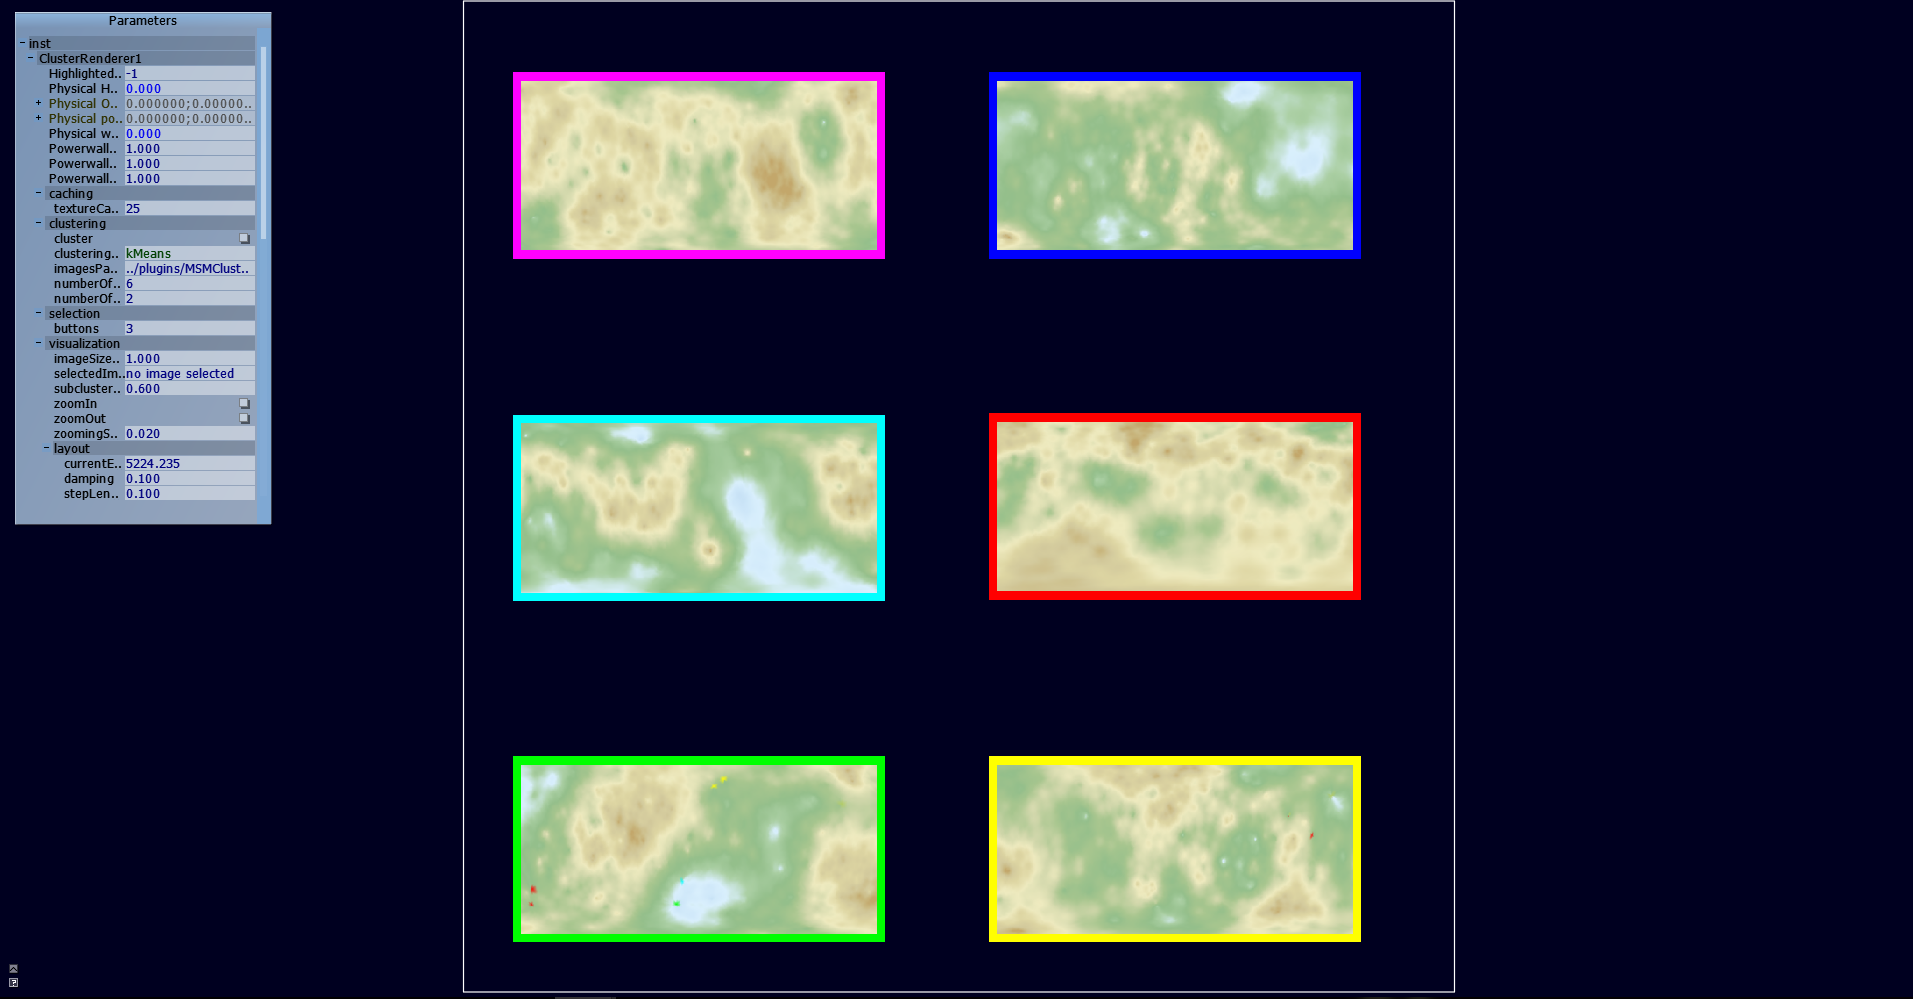
\includegraphics[width=12cm]{MegaMolExample.png}
\caption{Screenshot of a running MegaMol/MSMCLUSTER/comvi instance 
}\label{fig:teaser}
}

%%%%%%%%%%%%%%%%%%%%%%%%%%%%%%%%%%%%%%%%%%%%%%%%%%%%%%%%%%%%%%%%
%%%%%%%%%%%%%%%%%%%%%% START OF THE PAPER %%%%%%%%%%%%%%%%%%%%%%
%%%%%%%%%%%%%%%%%%%%%%%%%%%%%%%%%%%%%%%%%%%%%%%%%%%%%%%%%%%%%%%%%

\begin{document}

%% The ``\maketitle'' command must be the first command after the
%% ``\begin{document}'' command. It prepares and prints the title block.

%% the only exception to this rule is the \firstsection command
\firstsection{Introduction}\label{sec:intro}
%
\maketitle
%
\firstsection{Introduction} 
\todo{add sections to tasks in this section}%for journal use above \firstsection{..} instead
Over the span of 6 months we, the authors of this paper,  have researched and implemented a comparative clustering  process for images of molecular maps.
The task consisted of several parts: To generate images with the existing \verb|molecularmaps| plugin for MegaMol \cite{MegaMol} to build up a dataset, to extract a strong feature vector from the image, to find a way to cluster similar feature vectors and to visualize the clustering on the Powerwall with a tracking device.

This work was based on the MegaMol\cite{MegaMol} project. MegaMol is a simulation tool developed by the Universit\"at Stuttgart and the TU Dresden. It can be used to visualize particle data, simulations on atomic scale and other molecular processes such as the one that were presenting with our work. 
Due to its modular nature, it can be extended with modules to either build standalone plugins or build modules that interact and interface with each other.
In this paper we guide you through the \verb|MSMCLUSTER| plugin, its capabilities and inner workings.

One tasks was to retrieve molecular image data through existing MegaMol plugins \cite{molecularmaps}. For this a special binary of megamol was compiled and will be released in a separate project that will be publicly available starting \today \footnote{\url{https://github.com/aiosin/comvi}\\ Last retrieved: \today}.
The next task was to extract a expressive feature vector from those images and to find a metric to cluster them by similarity.

The last task which was also developed in a plugin in MagaMol was the visualization on the VISUS Powerwall. The Powerwall is a very high definition display \footnote{\url{https://www.visus.uni-stuttgart.de/institut/visualisierungslabor/technischer-aufbau.html} \\ Last retrieved: \today } that can be used to visualize large data(sets). Due to its size and resolution its possible to display much more information than on a regular consumer grade screen. 

The Powerwall also supports a tracker device that can transmit 6 degrees of freedom, so for the interaction step we had more possibilities than with  traditional human interface  devices  (HIDs), if you would exclude devices like smartphones. For this last step we also researched the possible interactions with the unique tracking device  which can be used  with the  Powerwall.

It is clear that the task required from us that we learn how to compare the images, measure the distances between the images, and cluster these images.
The given task required that we use a similarity based clustering algorithm.

Initially we were given the choice we could either chose to find similarities and cluster the proteins in the \verb|.pdb| format or given as bitmap image generated by the \verb|MolecularMaps| plugin in MegaMol \cite{molecularmaps}.

Since handling image files which give information about the protein in two dimensions was easier than dealing with the pdb file format which results in three dimensional visualizations we decided to start and carry out the task with the two dimensional approach.

To prevent confusion further down the paper  the reader should be familiar with the following two terms: comvi - internal name of the clustering engine that can be used by the MegaMol Plugin \\
MSMCluster - name of the Megamol plugin that was developed as the main part of the project 

Over the course of the next few pages you will learn how we approached these challenges and how we (attempted) solved them. You will find out what  worked and what didn't.

%-------------------------------------------------------------------------
\section{Related Work}\label{sec:relatedWork}

Clustering proteins by similarity or at least comparing individual proteins has been subject of existing work.

The paper \cite{kolesar} already had similar approaches to our results. Kolesar et al. used a 10 dimensional feature vector based on invariant image moments defined by Hu \cite{humoments}. Hu-Moments are set of invariant moments defined over a two dimensional signal, that give unique features about the the object in the image. More about image moments and the Hu Moments in section \ref{subsec:humom}.


Another approach for 3D protein data were 3D zernicke moments explored by La et al. in \cite{3dsurfer}. The approach is basically the same as in Kolesar et al. but La et al.  in \cite{3dsurfer} used Zernicke moments instead of traditional image moments and extended them to three dimensions. More about the comparison of the different methos in \ref{subsec:comparison}

For further information and more complex approaches to this problem one should consult the Smith Waterman algorithm from Smith and Waterman ``Identification of Common Molecular Subsequences''\cite{smithwater}. This work consideres the protein as a sequence of amino acids, rather than extracing two or three dimensional features over a two or three dimensional signal.\footnote{An overview can be found here: \url{https://www.ebi.ac.uk/Tools/sss/}}


\section{Clustering}
\todo{write some intrduction to clustering, aufteilen in subsections}
\subsection{Approaches to the Clustering-Problem}

Right of the start we had several ideas of how we could approach this problem. 
With the recent trend in machine learning we had a couple of ideas of how we could determine a similarity metric between two images or classify an image into a more usable vector of data.

We ended up using a higher dimensional feature vector described in \todo{give section label} to determine the similarirty between two protein maps because we didnt manage to train a custom model in the given timeframe, due to inexperience \todo{this can be said better}and non existance of labeled data.

But our relatively spartan results with a pretrained Imagenet \todo{cite imagenet} \cite{imagenet} \todo{cite darknet publication}  model let us to believe that given the knowledge on the subject and humanly labeled data (based on known featuresit \todo{LEFT OFF HERE}shoud be definetly possible for this specified task to find a machine learning  solution using neural networks/autoencoders.



\subsection{Finding a feature vector to cluster the images}

The challenge of finding a good feature vector was/is to find good features which are \todo{aussagekräfting} about the image.

The following procedure after finding/determining/calculating the feature vector for a given image is to apply some sort of dimensionality reduction to project a higher dimensional vector onto a 2D or 3D plane.

This has multiuple advantages. First If the dimensionality reduction works as intented one find out after applying the dimensionality reduction if similar looking items are positioned next to each other.

Another reason is the curse of dimensionality. As we all know in higher/infinite dimensional spaces, otherwise unexpected things start to happen such as the euclidian distance or mathimatically put the \begin{equation} L_2 \end{equation}-norm loses relevance since
\begin{equation}
\lim_{n\rightarrow \infty} x^n = 0 \quad \forall x \in [0,1)
\end{equation}

Simply put, otherwise very similar values get skewed to zero.

So we have to come up with other solutions to this problem discussed in \todo{put clustering section here}


\todo{back to finding the feature vector}
After looking at a small subset of molecular map images from a variety of proteins we determined that we needed to extract feature information about the follwoing properties of a given image: 

Color distribution, Shape, Texture and image moments 

The initial idea was that the color distribution gives information about the color palette in the image, the extracted shape features should give information about the the biggest \( n \) shapes in the picture, the texture feature should differentiate between smooth and rough texture and everything in between.

The image moments were chosen as a goto approach to extract invariant features from the image which has been proved to yield results as described in \cite{kolesar}

The exact image features that we extract from the image are the following:
\subsection{Image Features/Descriptors}
\subsection{Invariant Image Moments by Hu}\label{subsec:humom}

The set of invariant Image Moments discovered by Hu et. al \todo{find out if hu moments just him or others or et al.} are rotation, translation, scale and trasformation \todo{find out if correct} invariant. This allows us to determine if an image$I_a$ is similar to another image $I_B$ if $I_B$ is equal $I_A$ and simply rotated by $30^°$ \todo{put the value in degrees there}

The (continouus (spelling?)  Image ) Moments  over two dimensions at their core are defined as such:

\[m_{i,j} = \int^\infty_{- \infty}\int^\infty_{- \infty} f(x,y) dy dx \]. When dealing with discrete values like we find them in an (RGB/GS) Image we use sums insteads of integral so we get this:
\[m_{i,j} = \sum^n_{i=0}\sum^m_{j=0} f(i,y) \].\todo{get definition of moment}

Hu further defines his moments as such:

\todo{give the definition of all 7/8 moments (?) because this is going to take up a lot of space. }

Kolesar ended up using these moments \todo{put in kolsar moments}, in our case the moments \todo{put the hu moments here}

\subsection{Color palette/histogram }

The goal when extracting color palette was to reduce the big color space that is present in any of the molecular maps and get a few distinct \todo{aussagekräfting} colors from that range.

To achieve this we extract a histogram of each color channel of the RGB images. Each channel is then represented as a greyscale image. We then create for each channel a histogram of the luminance intensities with in our case 16 bins. This "reduces" the \(128*128 = 16384\) dimensions to just \(48\) dimensions for our image.

Alternatively you can take another approach described here

The results of both approaches will be discussed in \todo{cite}

\subsection{Texture}
\todo{better introduction}
After looking at a toy dataset of molecular maps we noticed that many samples had a distinct roughness that looked like they could be used to classify their texture.

We ended up using the haralick textural features. The haralick features work with a grey level correlation matrix (GCM). The gcm for a given greyscale image is defined as such:

\[\text{put the formula here, this is spaceholder}\]

Also we can take more features from that gcm than just the \todo{what exactly} can be taken from this matrix which gives us more features to work with.

we also computed this on every channel yielding us another \(x\) features \todo{expand texture features}.

Alternatively one can also use the tamura texture features. the tamura features are different to the haralick featues because they \todo{what exactly}.
They were primarily researched/developed/created to \todo{what exactly}. 	

\subsection{Shape}
We did not end up using the shape features described here but, since we spent quite some time getting them to work \todo{rephrase} I think it is important show how and why they were created.

The shape features we hoped to use were  fourier descriptors\footnote{\url{http://fourier.eng.hmc.edu/e161/lectures/fd/node1.html} } \footnote{\url{http://demonstrations.wolfram.com/FourierDescriptors/}}. In short, we get the centroid-distance curve of a distinct shape and take the fast (discrete) fourier transform of that curve. The technique has been proven to work for shape recognition  in earlier works \cite{fourierd}.

Our approach was the following.  Since our molecular maps are extremely complex (image-wise) we first need to divide the image into discrete image region.  We preferably want to segment our image into $n$ colors. To recap: our everyday monitor does support \(24\) bit colors, \(8 \) 8 bit per channel. that yields us \(2^{24}=16777216 \) colors.
We'd be lucky to find a countour in this color mess.
So our approach is to squash the color space down to a couple of colors.
This proces is called color segmenatation. We use the k means algorithm to put every 

Alternatively the mean-shift algorithm can be used. The algorithm is a kernel based clustering algorithm which operates sort of like the gradient descent algorithm.
Each point has a weight and initally all the points are laid out on a grid (or your dimensions next best spatial representation) each value attracts with a constant force all other neighboring values so they all suck each other in discrete clusters depending on the parameters (bandwith size and kernel weight) A comparison of color segmentation of mean shift and  k menas can be seen here. \todo{give image for comparison}

But our problem of color segmenatation was stil not solved. Especially in the k means algorithm we encountered a lot of smaller ``irrelevant'' shapes that we didnt want.
So one way of getting them out of the way was to squash the color space further down to two or three distint colors in the image.

Else we'd have to dynamically dilate and erode \todo{give link to dilation and erosion} the image until we can detect with a matrix labeling algorithm /  floodfill algorithm that we really have only a handful of shapes in the image.

For the shapes we then extract the contours and compute the centroid of that shape.
The centroid is the geometric center of mass of the shape or in other areas of science known as ..... the first moment 

Now we have the centroid and the countour of the shape that we want to classify we need to form the contour centroid distance curve.
The contour centroid distance curve is simply a disrete list of values of the contour \todo{clafiry} or the list of the euclidian (in two or three dimensions, why this doesnt work in higher dimensions look up \todo{curse of dimensionality}) distances.

We then normalize the values by diving all the values by the biggest value in the array, resulting in a array that is in range(0,1]

Without loss of generality depending on whhich curve we chose we take the fast discrete fourier transform of that signal, which gives us for each sine/cosine coefficient a weight how that component contributes/weighs in the signal.

Without any proof that would go beyond the scope of this paper we can say that the gained features are rotation scale and translation invariant. Its rotation invariant because ... its scale invariant because we normalize it, its translation invariant because the distance curve is translation invariant (wihtout proof).

Another shape feature can be won, if the shape object is given as a greyscale binary matrix. From this matrix one can extract Image Moment features like the one by Hu as described in \todo{give section to hu moments}

We did not end up using the shape features, because we could notice any improvement over the other features that we used, but it is important to note that they exist and what their capabilites are incase someone will continue our work on this topic. \todo{rephrase}.



\subsection{Finding the best performing similarity measure}

After our feature processing on an image we end up with an feature matrix where the rows are samples  and the columns are the features. aaaaa \[A \in \mathbb{R}\]


\subsection{Findin the best performign dimensionality reduction method}
For testing purposes we used every dimensionality reduction method we could find that looked halfway promising. We tested on datasets of various sizes and content.

We tested our results on the Oxford flower dataset and bmw dataset and our large (3000 images) molecular maps dataset and a medium version of that dataset (300 images) and a small dataset for fast testing purposes.

As you will find in our comvi repository \todo{give link} the dimensionality reduction routine consists of passing it a features array with \todo{beautify shape samples*features}
In the routine we additionally scale the data because \todo{why exactly ?!!??}.
We then return the reduced feature array back to the callee. The callee can then apply further some functions on this....

After inital testing with linear dimensionality reductions we notice that our results just wouldnt \todo{phrasing: converge }, so we again tried any non linear dimensionality reduction technique we could find.

We tested our data with LLE, MDS, kernel PCA, ISOMAP and t-SNE.
After testing with a small user group that would judge how good the clustering was done by the technique we concluded that t-SNE performed the best.

Further testing leads us to believe that t-SNE is the best dimensionality reduction procedure for this problem.

t-SNE is a randomized t bla Stochasitc neighbor embedding process. Its works by ... . But because the process requires random variables we decided to set the random seed of our program sowe can get deterministically the same results across different machines.

\subsection{Clustering - Algorithms and strategies }
\todo{this will be the main section for the clustering topic }
Because the given data was not labeled, only unsupervised machine learning techniques, like clustering, could be applied on it. 
Clustering of data is defined as the process of grouping n distinct values into m different classes. Clustering algorithm are algorithms that perform clustering. They can be subdivided in two different ways.
Depending on the number of classes to which one data element can belong we differ between hard and soft clustering. In hard clustering one element can belong to only one class, whereas in soft clustering it can belong to many different classes. 
On the other hand, depending on the way in which the data is clustered we differ between flat and hierarchical clustering. In flat clustering particular clusters have not relation to each other, whereas in hierarchical clustering considers the distance between clusters as well.

We applied the following clustering algorithms to image descriptors that were extracted from the protein images.

\begin{description}
\item [k-Means] K-Means takes the number of clusters as an input and if the data set contains more elements than the wanted number of clusters groups elements into that many clusters. Since it always groups data into the specified number of clusters k-Means is a flat clustering algorithm. Owing to the fact every image is clustered into only one cluster it belongs to hard clustering algorithms. 
To cluster the data k-Means uses the concept of centroids. Centroid is a point in vector space that is located in the middle of the corresponding cluster. There is therefore one centroid for every cluster. 
At first k-Means initializes the same number of centroids the same to the number of clusters. This can be done by choosing randomly that many points in the vector space. It then repeats reassignment and recomputation steps that behave as follows.
The main weakness of k-Means is that it does not converge to a global minimum. In order to circumvent this problem centroids are usually initialized randomly, but this then makes the algorithm non-deterministic.
MSMCluster plugin contains two implementations of k-Means. We implemented one version and the other version comes from the clustering part of the dlib library \cite{dlib09}.
\item [Hierarchical agglomerative clustering]
\item [Mean-shift]
\end{description}


There are several distinct clustering algorithm types. Hierarchical clustering, densitty based ..\todo{finish}


\subsection{Finding the best performing clustering algorithm}
Our approach to finding a clustering algorihtm was the same as the one that we used \todo{sentence and grammer  !!! } to find the best performing dimensionality reduction algorithm.

Except with a little modification. Kolesar et al. \cite{kolesar} used the k nearest neighbors algorithm over their 10-dimensional feature vector to cluster their data, as they discuss their results. We decided to further use this approach to cluster our molecular maps instead of the molecular protein tunnels which Kolesar et al. analyzed. \todo{phrasin}.


In the early stages of the projcet we intended to use the DBSCAN clustering algoirtm. 
The key feature to this algorithm is that it automatically determines the optimal number of clusters that it detects in the given data. 

The algorithm is a density based spatial clustering algirhtm that uses a similarity metric between two items that are to be  clustered defined over the domain \([0,1]\). So the ways of computing the similarity is given more freedom with this approach.


You could use the euclidian distance between two feature vectors or the cosine distance or feed the two images to a siamese neural network/autoencoder \todo{give information about siamese neural networks and autoencoders} which will have learned the similarity metric between the images.

You could also usethe householder/hausdorff distancebetween two higher dimensional vectors.

We opted against DBSCAN for our primary clustering algorithm because in the early stages of the project the computation of the \(nxn\) similarity matrix was very computationally expensive and took quite a bit more time than the approaches that we demonstrate in the next paragraphs

There are similar approaches \todo{finish sentence}

For our testing we used k nearest neighbors with the elbow method and a cutoff at  ~85 \% \todo{what exactly}

spectral clustering, chinese whispers  ... 

We ended up with the mean shift algorithm. It also is a density based algorithm and much like the DBSCAN algorithm is also determines the optimal number of clusters for the given parameters but it operates with a kernel sampled on each point in the plot and calculates the center of mass so to speak of the points clouds, for a animated demonstration lookt at \todo{give link to mean shift visualization}. For a demonstration of the mean shift algorithm look at Figure \ref{fig:tsne}. 




\subsection{Testing the feature vector with other datasets}
\begin{figure}[tb]
	\begin{center}
		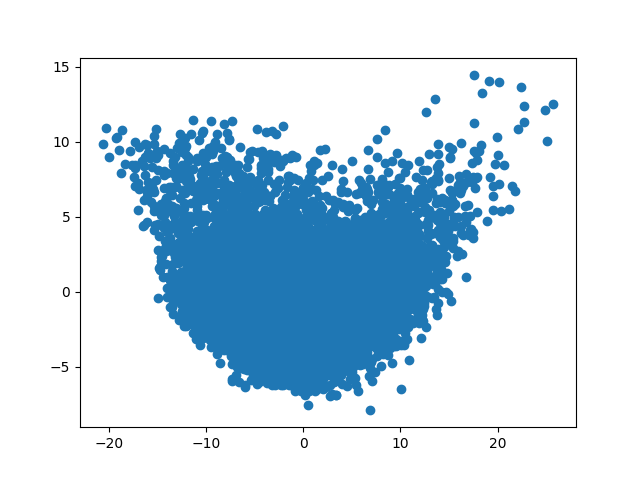
\includegraphics[width=.75\linewidth]{Figure1.png}
	\end{center}
	\caption{\label{fig:lorem} Early test wihh the Oxford flower dataset \todo{cite oxford flower dataset}}
\end{figure} 
\begin{figure}[tb]
	\begin{center}
		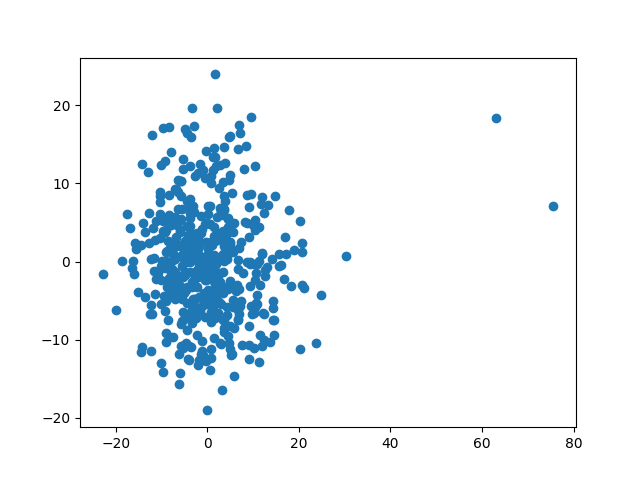
\includegraphics[width=.75\linewidth]{Figure2.png}
	\end{center}
	\caption{\label{fig:bmw} Early test with the bmw car dataset \todo{cite stanford car dataset}\cite{stanfordcar}}
\end{figure}
\begin{figure}[tb]
	\begin{center}
		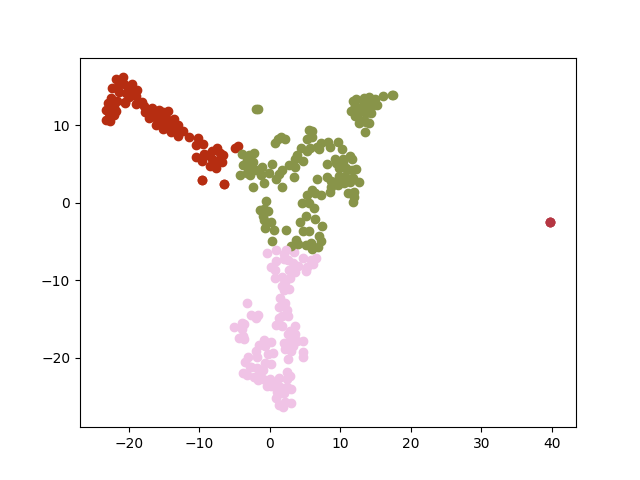
\includegraphics[width=.75\linewidth]{MS-tsne.png}
	\end{center}
	\caption{\label{fig:tsne} final test with the tsne dimensionality reduciton and the mean shift clustering algorithm }
\end{figure}

\begin{figure}[tb]
	\begin{center}
		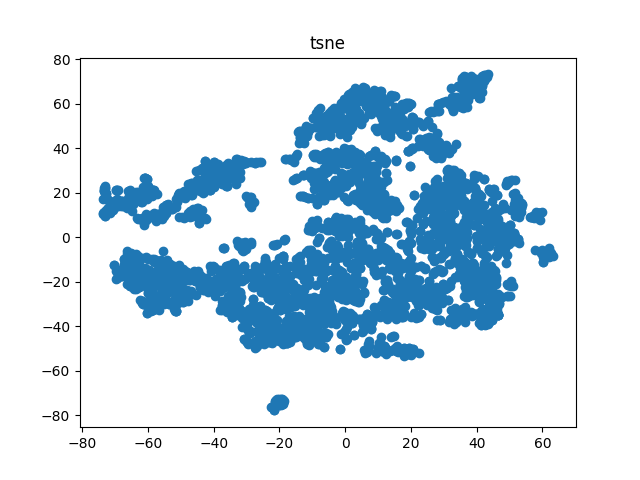
\includegraphics[width=.75\linewidth]{tsneFull.png}
	\end{center}
	\caption{\label{fig:tsnef} final test with the tsne dimensionality reduciton and the mean shift clustering algorithm }
\end{figure}

\section{Visualization and Interaction}
\todo{write some introduction about Powerwall, trackingsystem, visus etc.}

\subsection{Approaches to the Visualization-Task}

Our aproaches to visualizing the given clusters were the following, the reader is reminded that we are not just visualizing the clusters on a ''normal machine'' but rather the Powerwall, a projected display with effectively 6-24 times the resolution of a consumer grade display. Details on the Powerwall can be found \todo{cite Powerwall publicatoin here if available}. \cite{Powerwall}

If we are given so much pixel real estate we are given the freedom to draw smaller pixels since we still will be able to see them on the Powerwall.

During the duration of the project the idea of a 3D visualization was discussed among the team, but we settled for a 2D visualization. This had a couple of reasons.

While the interactions with the data in 3D would have been more fun since we had more degrees of freedom to work with.
But we could not find a way to present the data in a way such that with just a glance the user could intuitively interpret the data that would be displayed on the screen.

... So we decided to settle for a 2D visualization. Our approach is rather boring but it works. On startup we display nothing, if the user chooses his supplied image data and the algorithms used to cluster the pictures he gets the option to start the visualization.

The visualizatoin consists of displaying the image of a cluster representative with a simple rectangle. 
This way the user knows exactly what to expect to be in the cluster.

If the user wishes to have a closer look at the images in the given cluster he can click onto the representative and will get a view of all the images in that cluster.

We decided after testing with toy test and real datasets that one level of subclustering is enough, after 2 levels of subclustering the clusters get \todo{find better expression}  noisy and ambiguous.

In both the main and subcluster view the representatives are visualized with "force directed layout", to avoid 



\subsection{Approaches to the Interaction with and mouse and the Powerwall tracking stick (?) \todo{cite correct pub and use correct name}}

\todo{@shoma @enis @damir interaktionsmöglichkeiten schreiben}
\todo{rephrase}
The tracking system that was provided to us from the VISUS of the University of Stuttgart was the \todo{motive imsys (?)} tracking system which uses the \todo{vrpn natnet} protocol to send the interaction from the 6 DOF stick in the three dimensions to the client machine. 
Since we are visualizing the data in two dimensions we have at least one spatial dimension that can be repurposed for secondary/other uses rather than tracking the position of the stick from world coordinates into screen coordinates.

The tracking stick also has two buttons that can be interacted with yielding a total of 4 buttons states (off off, off on, on off, on on ) that can be used.

Our design process of the interactions was first  laying out all of the possible actions that we wanted to cover and then experimentally incorporating them in to the implementation.

We wanted to be able to 
\begin{enumerate}
  \item have a cursor 
  \item zoom into the picture and  explore the different clusters
  \item navigate into a cluster
  \item display a cluster as a gridview if a) the cluster size allowed this and b)there was enough screen real estate available for this.
  
\end{enumerate}
\subsection{Approaches to the Visualization-Task}

Our aproaches to visualizing the given clusters were the following, the reader is reminded that we are not just visualizing the clusters on a ''normal machine'' but rather the Powerwall, a projected display with effectively 6-24 times the resolution of a consumer grade display. Details on the Powerwall can be found \todo{cite Powerwall publicatoin here if available}. \cite{Powerwall}

If we are given so much pixel real estate we are given the freedom to draw smaller pixels since we still will be able to see them on the Powerwall.

During the duration of the project the idea of a 3D visualization was discussed among the team, but we settled for a 2D visualization. This had a couple of reasons.

While the interactions with the data in 3D would have been more fun since we had more degrees of freedom to work with.
But we could not find a way to present the data in a way such that with just a glance the user could intuitively interpret the data that would be displayed on the screen.

... So we decided to settle for a 2D visualization. Our approach is rather boring but it works. On startup we display nothing, if the user chooses his supplied image data and the algorithms used to cluster the pictures he gets the option to start the visualization.

The visualizatoin consists of displaying the image of a cluster +representative with a simple rectangle. 
This way the user knows exactly what to expect to be in the cluster.

If the user wishes to have a closer look at the images in the given cluster he can click onto the representative and will get a view of all the images in that cluster.

We decided after testing with toy test and real datasets that one level of subclustering is enough, after 2 levels of subclustering the clusters get \todo{find better expression}  noisy and ambiguous.

In both the main and subcluster view the representatives are visualized with "force directed layout", to avoid 

\subsection{Approaches to the Interaction with and mouse and the Powerwall tracking stick (?) \todo{cite correct pub and use correct name}}

\todo{@shoma @enis @damir interaktionsmöglichkeiten schreiben}
\todo{rephrase}
The tracking system that was provided to us from the VISUS of the University of Stuttgart was the \todo{motive imsys (?)} tracking system which uses the \todo{vrpn natnet} protocol to send the interaction from the 6 DOF stick in the three dimensions to the client machine. 
Since we are visualizing the data in two dimensions we have at least one spatial dimension that can be repurposed for secondary/other uses rather than tracking the position of the stick from world coordinates into screen coordinates.

The tracking stick also has two buttons that can be interacted with yielding a total of 4 buttons states (off off, off on, on off, on on ) that can be used.

Our design process of the interactions was first  laying out all of the possible actions that we wanted to cover and then experimentally incorporating them in to the implementation.

We wanted to be able to 
\begin{enumerate}
  \item have a cursor 
  \item zoom into the picture and  explore the different clusters
  \item navigate into a cluster
  \item display a cluster as a gridview if a) the cluster size allowed this and b)there was enough screen real estate available for this.
  
\end{enumerate}



\section{Discussion of results}
As we saw on the last few pages, we have written a plugin for MegaMol that takes pdb datafile or already generated molecular maps as an input and clusters  the corresponding individual protein maps by similarity.

\subsection{comparing our findings with other protein similarity practices}\label{subsec:comparison}
Laa di daa bla blubb I am a placeholder aylmao, look at me. bla \cite{3dsurfer} blah protein database simlilarity measure.


\begin{table}
  \caption{
  \label{tab:perf} placeholder comparisons of different protein similarity comparisons/algorithms}
  \centering
  \vspace{0.3em}
  \begin{tabular}{lrr}
  dataset & full performance (fps) & half performance (ms)\\ \hline\\[-0.4em]
  big (3k images) & 1,243 & 0.1 \\
  medium (300 image ) & 23 & 23 \\
  small (~12 images) & 23,312,134.3 & 22.1 \\
  \end{tabular}
  \end{table}



\section{Conclusion}


%% if specified like this the section will be ommitted in review mode
\acknowledgments{
We would like to thank our supervisors Michael Krone and Florian Fries as well as our project examiner Prof. Ertl, for giving us this opportunity to work on this project. We are grateful that we were able to improve our knowledge and learn new things. We are also grateful for the feedback we recieved on our work. \\
This work was partially funded by cake and cookies.
}

\bibliographystyle{abbrv}
%%use following if all content of bibtex file should be shown
%\nocite{*}
\bibliography{comvi}
\end{document} 
